% Copyright 2024 Adam Christiansen
% SPDX-License-Identifier: LPPL-1.3c
%
% This file may be distributed and/or modified under the conditions of the
% LaTeX Project Public License (LPPL), either version 1.3c of this license or
% (at your option) any later version. The latest version of this license is in
% the file
%
%    https://www.latex-project.org/lppl.txt
%
% This file (The Work in the LPPL) can be distributed on its own.
%
% This file can be found at
%
%    https://github.com/adamchristiansen/latex-stz
%

\documentclass[10pt,titlepage]{article}

\usepackage{tabularx}
\usepackage[hidelinks]{hyperref}

\usepackage{stz}

\tcbuselibrary{listings}

\title{\texttt{stz}}
\author{Adam Christiansen}
\date{\today}

% How to render the name of a LaTeX package.
\newcommand*{\packagename}[1]{\texttt{#1}}

% How to render inline code.
\newcommand*{\code}[1]{\texttt{#1}}

% Show LaTeX code and its result side by side.
\NewTCBListing{example}{ !O{} }{%
  % Spacing.
  boxsep=0pt,
  left=0pt,
  right=0pt,
  % Frame.
  enhanced,
  frame hidden,
  boxrule=0pt,
  lower separated=false,
  sharp corners,
  % Color.
  colback=white,
  % Layout.
  listing side text,
  halign upper=justify,
  halign lower=justify,
  % Extras.
  #1
}

\begin{document}

\maketitle
\tableofcontents
\clearpage

%==============================================================================
% Purpose
%==============================================================================

\section{Purpose}

I found myself often rewriting the same macros and configurations
over and over again every time I create a new document.
This package is my consolidated set of utilities
and opinionated set of styles and tweaks.
This document serves as a limited showcase
and set of quick visual test cases for the \code{stz} package;
This document does not give examples of every feature,
and \code{stz.sty} should be read for the full list of features.

\begin{caution}
  This package is not stable and can change at any time.
\end{caution}

%%%%%%%%%%%%%%%%%%%%%%%%%%%%%%%%%%%%%%%%%%%%%%%%%%%%%%%%%%%%%%%%%%%%%%%%%%%%%%%
%%%  _______                 _
%%% |__   __|               | |
%%%    | |_      _____  __ _| | _____
%%%    | \ \ /\ / / _ \/ _` | |/ / __|
%%%    | |\ V  V /  __/ (_| |   <\__ \
%%%    |_| \_/\_/ \___|\__,_|_|\_\___/
%%%
%%%%%%%%%%%%%%%%%%%%%%%%%%%%%%%%%%%%%%%%%%%%%%%%%%%%%%%%%%%%%%%%%%%%%%%%%%%%%%%

\section{Tweaks}

Tweaks are adjustments to LaTeX itself or external packages.

%==============================================================================
% Floats
%==============================================================================

\subsection{Floats}

The \code{table} and \code{figure} environments are adjusted to use
\code{t!} positioning and \code{\string\centering} by default.

%==============================================================================
% xcolor
%==============================================================================

\subsection{\packagename{xcolor}}

The 19 standard colors provided by \packagename{xcolor} are redefined and are
the only colors used throughout this package.

\newcommand*{\swatch}[1]{\tikz{
  \draw[draw=#1!75!black,fill=#1,thick]
    (-0.75\baselineskip,-0.5\baselineskip) rectangle (0.75\baselineskip,0.5\baselineskip);
  \node[anchor=west] at (0.75\baselineskip,0) {\texttt{\strut#1}};
}}

\noindent
\begin{tabularx}{\textwidth}{@{}XXX@{}}
  \swatch{black}     & \swatch{red}    & \swatch{blue}    \\
  \swatch{darkgray}  & \swatch{orange} & \swatch{violet}  \\
  \swatch{gray}      & \swatch{yellow} & \swatch{purple}  \\
  \swatch{lightgray} & \swatch{lime}   & \swatch{magenta} \\
  \swatch{white}     & \swatch{green}  & \swatch{pink}    \\
  {}                 & \swatch{teal}   & \swatch{brown}   \\
  {}                 & \swatch{cyan}   & \swatch{olive}   \\
\end{tabularx}

%==============================================================================
% siunitx
%==============================================================================

\subsection{\packagename{siunitx}}

These are tweaks to the \packagename{siunitx} package.

\begin{example}
% Lists, products, and ranges use a single unit and an Oxford comma.
\qtylist{1;2;5;10}{\mm}
\end{example}

\begin{example}
% Math mode is allowed in numbers.
\qty{\sim100}{\nano\volt}
\end{example}

\begin{example}
% Uncertainty is compact.
\qty{12345(67)}{\micro\ampere}
\end{example}

\begin{example}
% Powers are used when there is more than one denominator.
\qty{1}{\metre\per\second} \\
\qty{1}{\watt\per\metre\per\kelvin}
\end{example}

\begin{example}
% Several qualifiers are provided.
\qty{1}{\volt\rms}
\end{example}

%==============================================================================
% TikZ and PGF
%==============================================================================

\subsection{Ti\textit{k}Z and PGF}

Several defaults are changed for \packagename{tikz} and \packagename{pgf}.
The most apparent are plots.

{
\pgfplotsset{height=1.25\linewidth}
\begin{example}
\pgfplotsset{domain=0:1,samples=6}
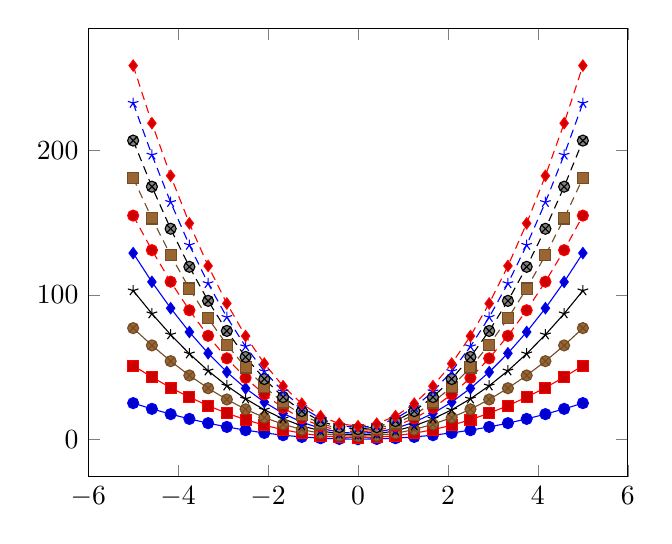
\begin{tikzpicture}
  \begin{axis}
    \addplot+ { 1*x^2+0};
    \addplot+ { 2*x^2+1};
    \addplot+ { 3*x^2+2};
    \addplot+ { 4*x^2+3};
    \addplot+ { 5*x^2+4};
    \addplot+ { 6*x^2+5};
    \addplot+ { 7*x^2+6};
    \addplot+ { 8*x^2+7};
    \addplot+ { 9*x^2+8};
    \addplot+ {10*x^2+9};
  \end{axis}
\end{tikzpicture}
\end{example}
}

%%%%%%%%%%%%%%%%%%%%%%%%%%%%%%%%%%%%%%%%%%%%%%%%%%%%%%%%%%%%%%%%%%%%%%%%%%%%%%%
%%%  ______ _                           _
%%% |  ____| |                         | |
%%% | |__  | | ___ _ __ ___   ___ _ __ | |_ ___
%%% |  __| | |/ _ \ '_ ` _ \ / _ \ '_ \| __/ __|
%%% | |____| |  __/ | | | | |  __/ | | | |_\__ \
%%% |______|_|\___|_| |_| |_|\___|_| |_|\__|___/
%%%
%%%%%%%%%%%%%%%%%%%%%%%%%%%%%%%%%%%%%%%%%%%%%%%%%%%%%%%%%%%%%%%%%%%%%%%%%%%%%%%

\section{Elements}

Elements are new features.

%==============================================================================
% Admonitions
%==============================================================================

\subsection{Admonitions}

Admonitions provide highlighted notes with context.

\begin{example}
\begin{note}
  A note that stands out.
\end{note}
\end{example}

\begin{example}
\begin{tip}
  Optional tip.
\end{tip}
\end{example}

\begin{example}
\begin{important}
  Important information.
\end{important}
\end{example}

\begin{example}
\begin{caution}
  Potential risk.
\end{caution}
\end{example}

\begin{example}
\begin{danger}
  Negative consequences.
\end{danger}
\end{example}

%==============================================================================
% Todo
%==============================================================================

\subsection{Todo}

% Todo notes emit warnings. The uses of todo in this section are intended and
% the warnings will not be legitimate, so warnings are temporarily disabled
% then enabled again at the end of the section.
\makeatletter
\let\old@stz@warning\@stz@warning
\let\@stz@warning\@gobble
\makeatother

Add todo notes to indicate work that must still be done.
All todo notes emit warnings in the log.

\begin{example}
\begin{todo}
  A big note.
\end{todo}
\end{example}

\begin{example}
Highlight \todoadd{text} to add.
\todoadd{}
\end{example}

\begin{example}
Highlight \todoremove{text} to remove.
\todoremove{}
\end{example}

\begin{example}
Highlight \todofix{text} to fix.
\todofix{}
\end{example}

\begin{example}
Highlight \todorevise{text} to revise.
\todorevise{}
\end{example}

\begin{example}
A \todocite{citation} is required.
\todocite{}
\end{example}

\begin{example}
Cross \todoref{reference} required.
\todoref{}
\end{example}

\begin{example}
More \todomore{text} required.
\todomore{}
\end{example}

\begin{example}
% Can include optional number of sentences.
\todosentence
% \todosentence[2]
\end{example}

\begin{example}
% Can include optional number of paragraphs.
\todopar
% \todopar[2]
\end{example}

{
\stzsetup{todo/box/.cd,height=2.5cm,width=\linewidth}
\begin{example}
% Useful for placeholder figures and tables.
\todobox
\end{example}
}

% Enable warnings again.
\makeatletter
\let\@stz@warning\old@stz@warning
\let\old@stz@warning\undefined
\makeatother

\end{document}
